\subsection{$\gamma$ + Jet Measurements}
\label{sec:res_gjet}

As for dijets, the measurement of the jet \pt resolution using the $\gamma+$jet \pt-balancing, involves an extrapolation of the event 
topology  to the ideal case of zero secondary hadronic activity, as described in detail in Section~\ref{sec:radbias}. To measure the jet \pt resolution from data, the observable $\sigma(\pt^{Jet}/\pt^{\gamma})$ is expressed as: 

\begin{equation}
   \sigma_{total}(\pt^{Jet}/\pt^{\gamma}) =  \sigma_{intrinsic}(\pt^{Jet}/\pt^{gen}) \oplus \sigma_{imbalance}(\pt^{gen}/\pt^{\gamma}),
\end{equation}

where the first term $\sigma_{intrinsic}(\pt^{Jet}/\pt^{gen})$ is the intrinsic (generator-level MC) resolution of interest. The second term $\sigma_{imbalance}(\pt^{gen}/\pt^{\gamma})$ is the ``imbalance'' term, arising from the presence of secondary jets in an event and from other effects, such as hadronization. The effect of extra jet activity is studied as a function of $\pt^{Jet2}/\pt^{\gamma}$. 

The jet \pt resolution is measured using two methods. The ``direct'' method measures the \pt resolution separately for data and MC, while the ``ratio'' method is specialized for the data/MC ratio. In the direct method, the intrinsic resolution is  taken to be independent of $\pt^{Jet2}/\pt^{\gamma}$, while the width of the imbalance is assumed to be a first-order polynomial in the 
$\pt^{Jet2}/\pt^{\gamma}$ fraction. The intercept ``$q$'' gives the limit of zero secondary jet activity and the parameter ``$m$'' describes the soft-radiation effects:

\begin{equation}
   \sigma_{intrinsic}(\pt^{Jet2}/\pt^{\gamma}) = c,
\end{equation}

\begin{equation}\label{eq:imb}
   \sigma_{imbalance} (\pt^{Jet2}/\pt^{\gamma}) = q + m \cdot \pt^{Jet2}/\pt^{\gamma},
\end{equation}

\begin{equation} \label{eq:totalRes}
   \sigma_{total} (\pt^{Jet2}/\pt^{\gamma}) = \sqrt{(c^2 + q^2 + 2qm \pt^{Jet2}/\pt^{\gamma}+m^2(\pt^{Jet2}/\pt^{\gamma})^2)}\,.
\end{equation}

In order to correct for the particle-level imbalance, the measured \pt resolution, using reconstructed jets and photons, is fitted with the functional form in Eq.~(\ref{eq:totalRes}), while keeping the parameter $q$ fixed to the value obtained from the fit to the imbalance in MC, using the functional form in Eq.~(~\ref{eq:imb}). A non-zero value of the intercept $q$ is expected, which represents the irreducible imbalance due to, e.g. hadronization and photon resolution effects. The parameter $c$ is the measured intrinsic resolution from the reconstructed quantities. The same functional form is used in fits to both MC and data samples.

Figure~\ref{fig:GenPtRecPhotRes} (left) shows $\pt^{jet}/\pt^{\gamma}$ distributions, for different bins of $\pt^{Jet2}/\pt^{\gamma}$, in MC simulation. The effect of tightening the secondary jet activity is clearly visible as a narrowing of the spread of the  distributions. The intrinsic resolution on the other hand, is independent of any other activity in the event. The evolution of the 
RMS of the \pt-balance distribution in bins of $\pt^{Jet2}/\pt^{\gamma}$ is shown in Fig.~\ref{fig:GenPtRecPhotRes} (right) as the red circular points, for both data and MC samples. The blue square points show the intrinsic resolution of PF  jets in MC simulation, measured as the RMS of the $\pt^{PFJet}/\pt^{gen}$. The grey thicker line shows the total expected resolution defined as the quadrature sum of intrinsic (blue square points) and imbalance component (green triangle points), as a function of $\pt^{Jet2}/\pt^{\gamma}$. The dotted-red line is the result of the fit, applied to MC simulation, and the thinner solid-red line is the functional fit to the data measurement.

\begin{figure}[htbp]
\begin{center}
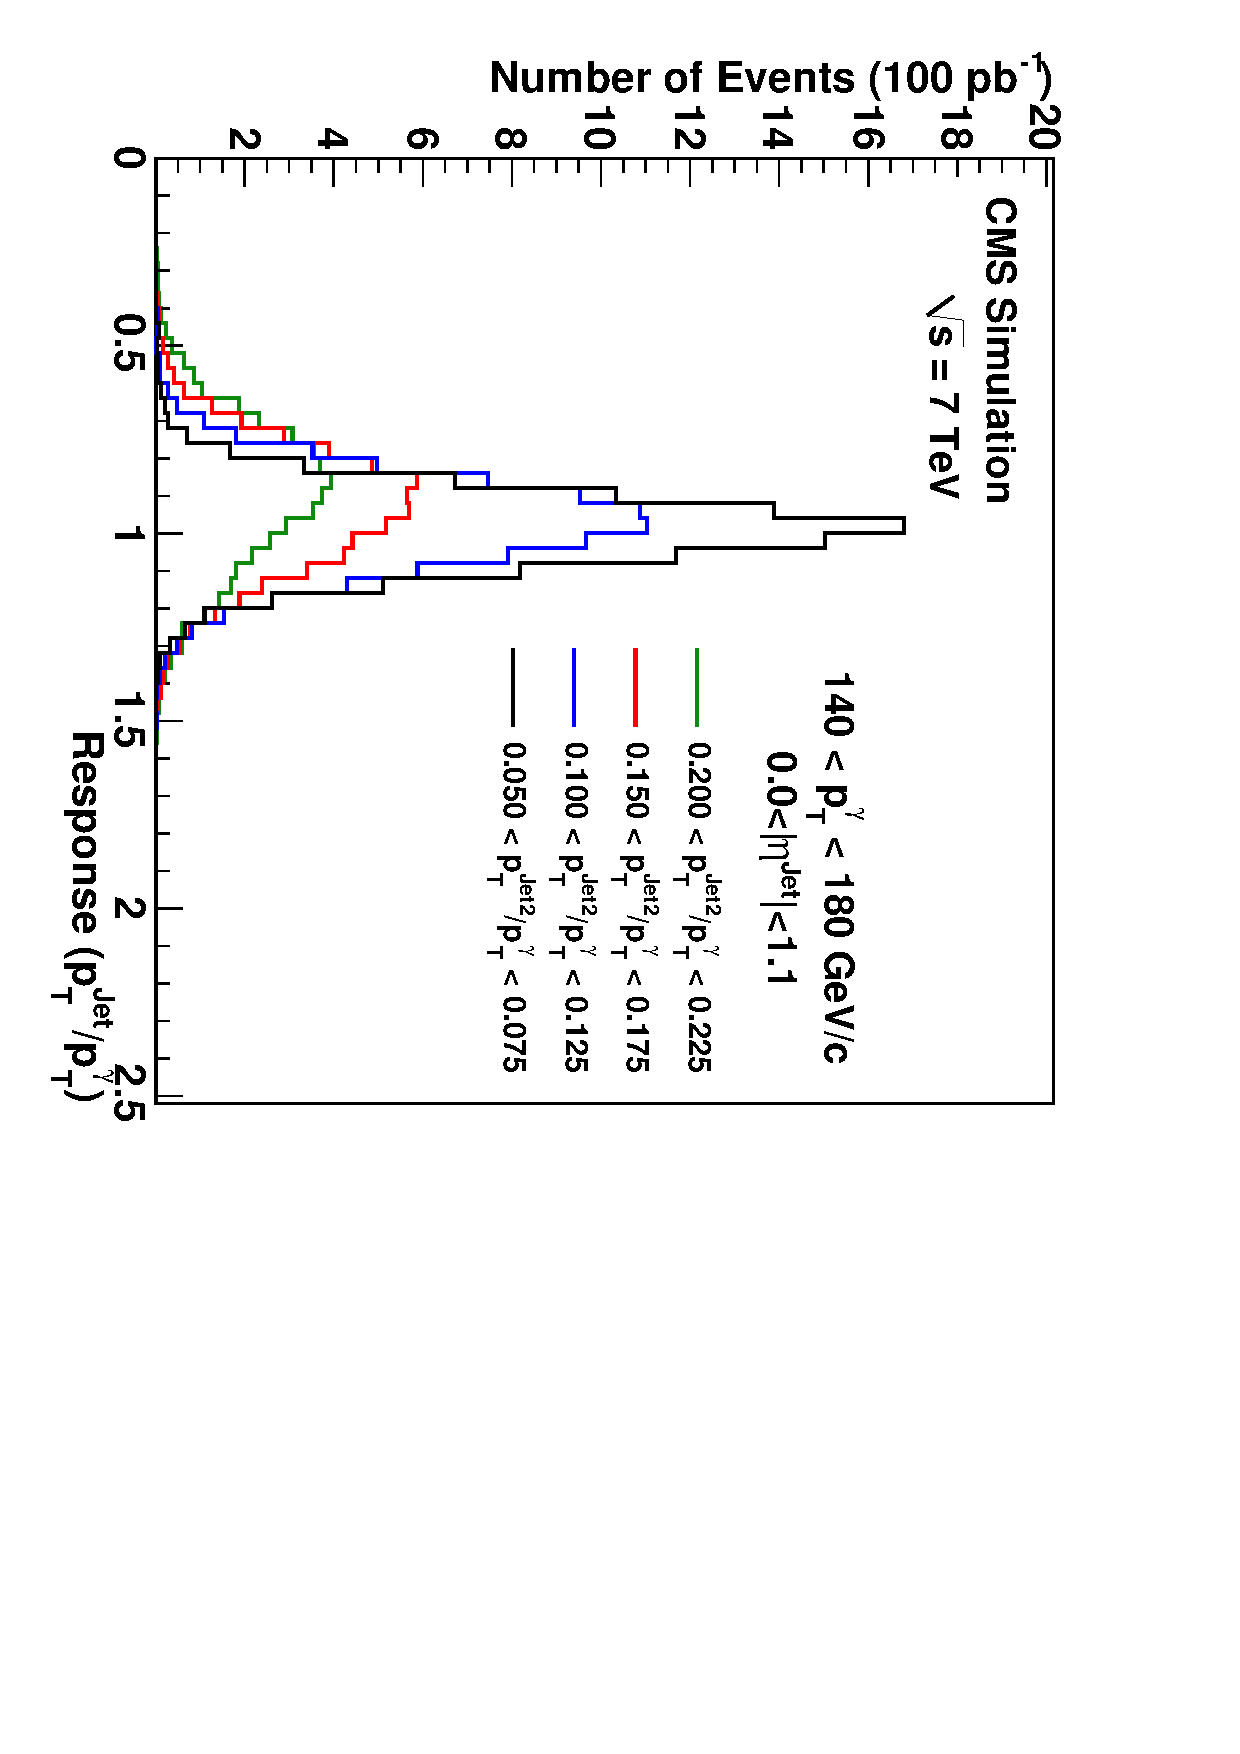
\includegraphics[angle=90,width=0.48\textwidth]{Figures/JER/figs/res_photon/c_MeasRecJetRecPhot_ptBin7_etaBin1.pdf}
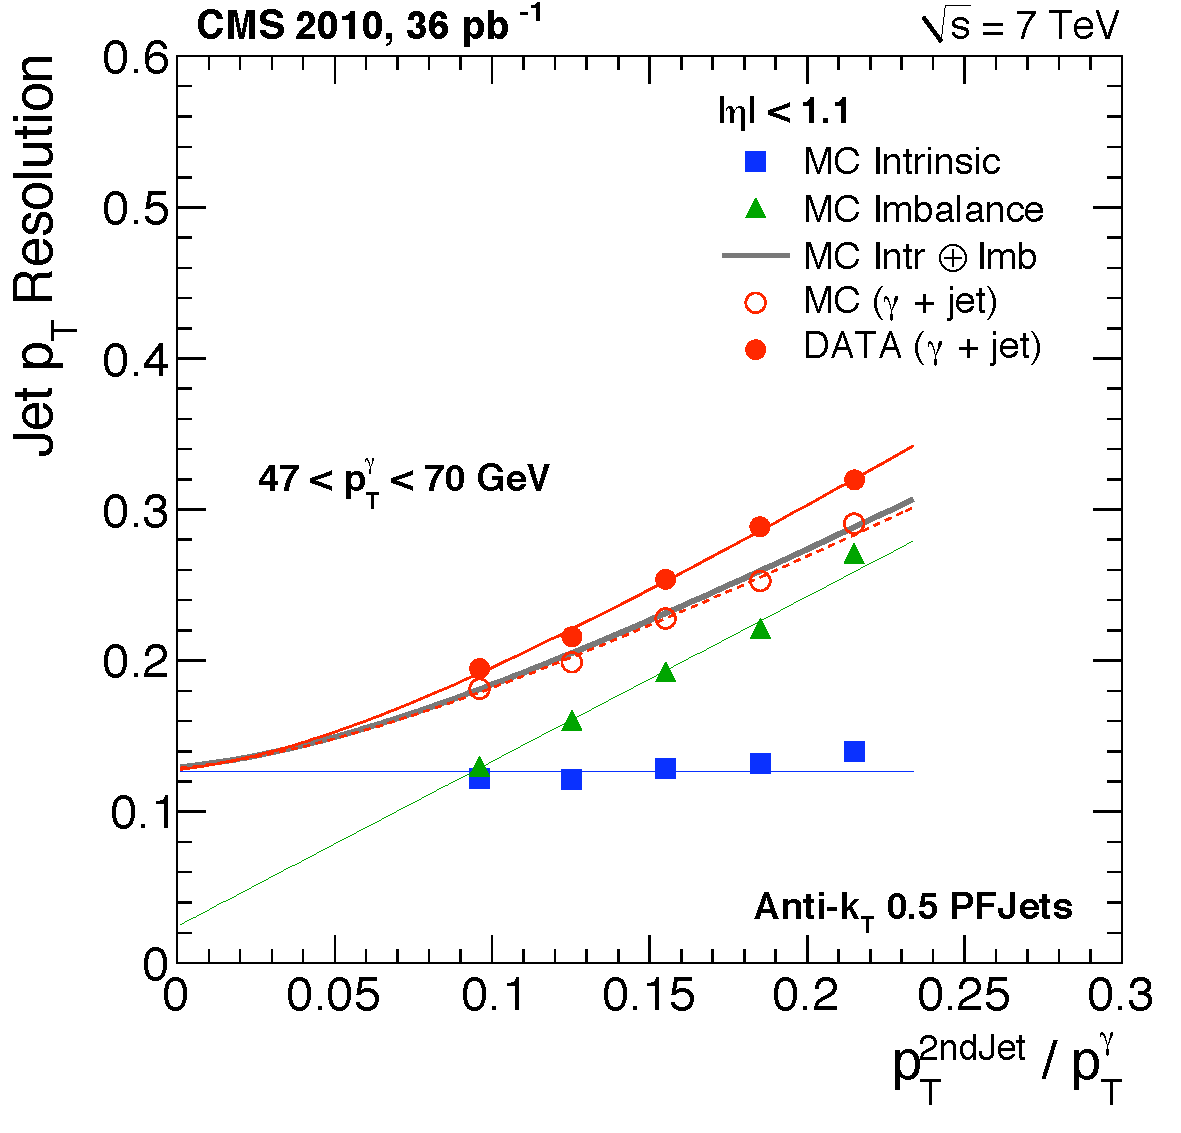
\includegraphics[width=0.48\textwidth]{Figures/JER/figs/res_photon/resolutionL2L3_eta011_ptBin_47_70_RecoRelRaw.pdf}
\end{center}
\caption[]{Response distributions in different bins of $\pt^{Jet2}/\pt^{\gamma}$, and for $140<\pt^{\gamma}<180\GeV$ (left), components of the jet \pt resolution, as a function of $\pt^{Jet2}/\pt^{\gamma}$ for PF jets in data and MC samples (right).}
\label{fig:GenPtRecPhotRes}
\end{figure}

The $\gamma+$jet sample has significant contamination from QCD dijet background with a jet misidentified as a photon. To pass the photon isolation and cluster shape requirements, such a jet must be composed of a leading $\pi^0$ (with $\pi^0 \to\gamma\gamma$) accompanied by a very low hadronic activity. These misidentified ``photons'' have energy-scale similar to the genuine prompt photons, a good energy resolution, and can therefore serve as valid reference objects for this analysis. In the selected photon sample, the presence of a jet is required, with $|\eta|<1.1$, recoiling against the photon candidate in azimuth within $\Delta \phi > 2\pi/3$. 

Distributions of the $\pt/\pt^{\gamma}$ variable for PF jets are shown in Fig.~\ref{fig:response} for data and MC. The distributions are not centered around the response of 1.0, because of the impact of soft radiation, as illustrated in Fig.~\ref{fig:GenPtRecPhotRes}.

\begin{figure}[t]
\centering
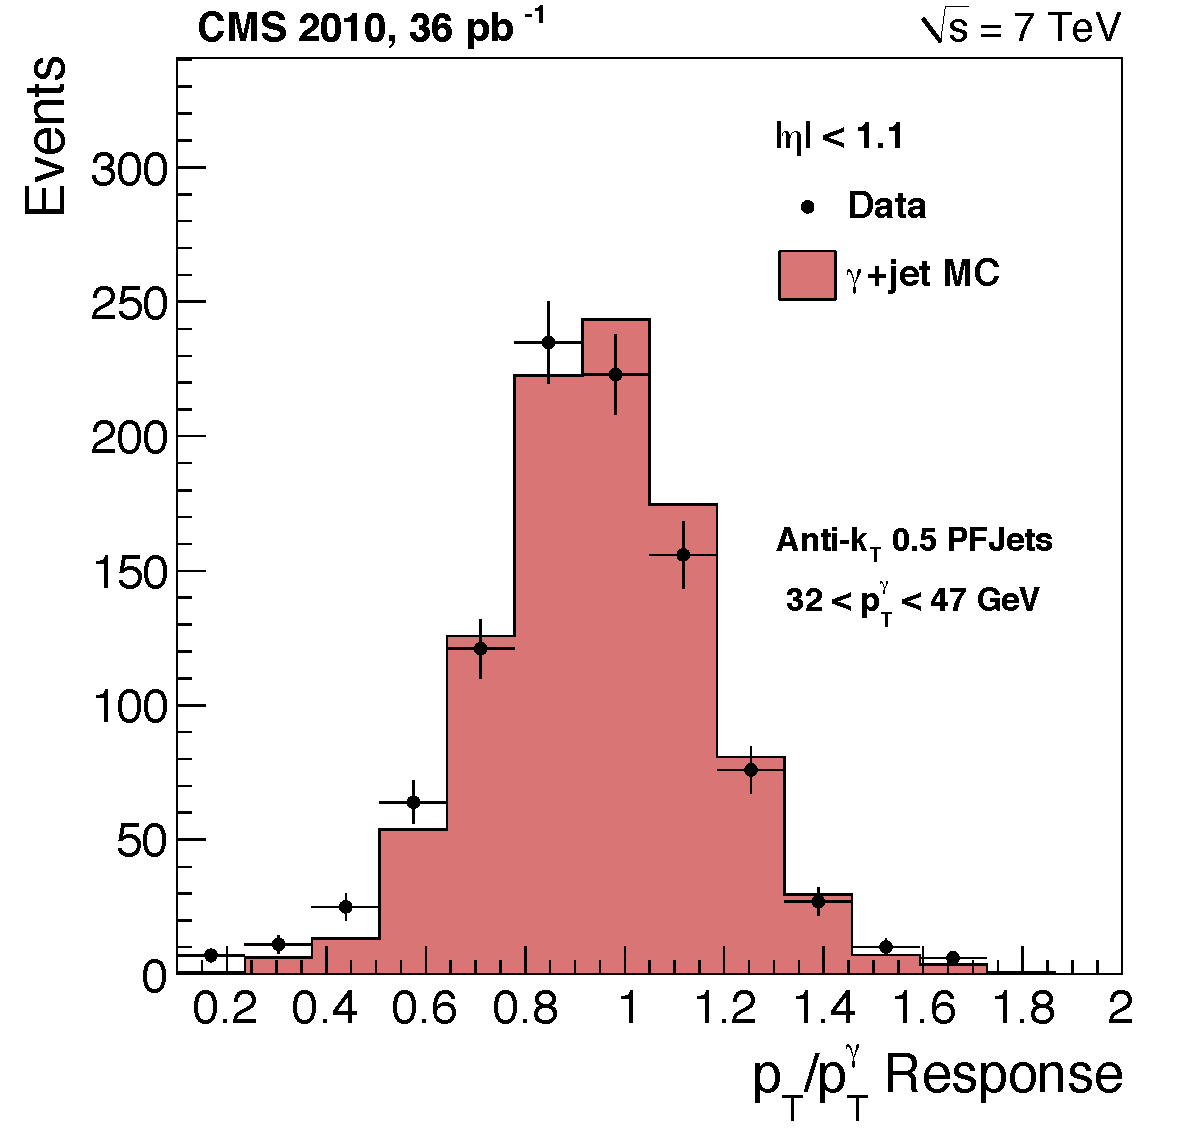
\includegraphics[width=0.49\textwidth]{Figures/JER/figs/res_photon/response_L2L3_eta011_ptPhot_32_47}
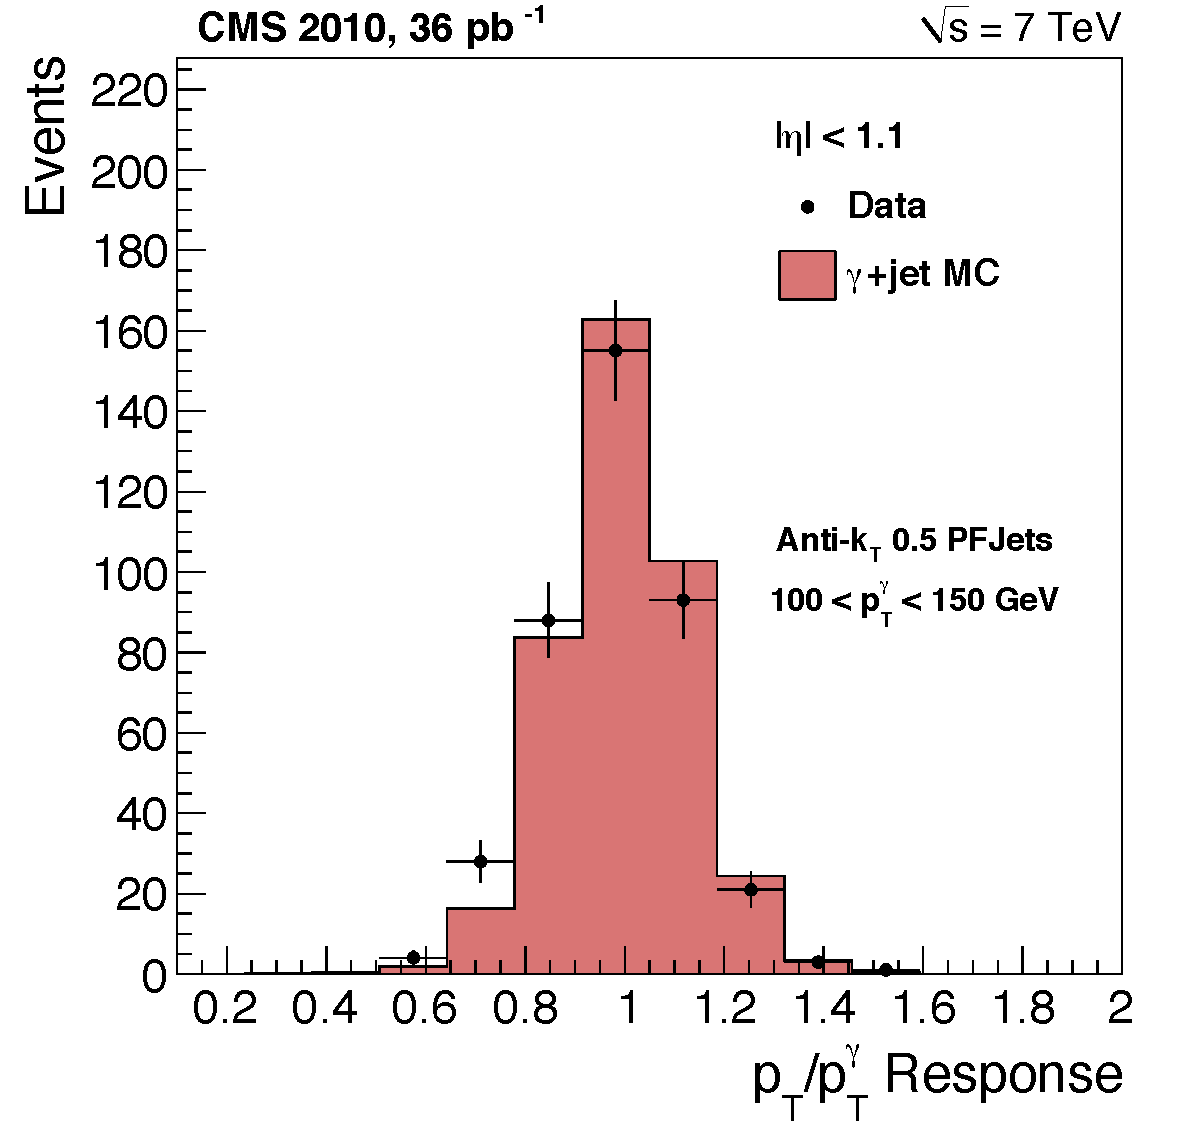
\includegraphics[width=0.49\textwidth]{Figures/JER/figs/res_photon/response_L2L3_eta011_ptPhot_100_150}
\caption{Distributions of $\pt/\pt^{\gamma}$ in data and MC sample for PF jets in two representative $\pt^{\gamma}$ bins.}
\label{fig:response}
\end{figure}

The jet \pt resolution obtained from the $\gamma+$jet analysis, 
provides a cross-check of the dijet asymmetry results, and a 
reasonable agreement is observed between the two measurements, as 
shown in Fig.~\ref{fig:gammajet_dijet}. At the current level of statistics, 
the $\gamma+$jet method  yields poorer resolutions for $\pt>150\GeV$.

\begin{figure}[t]
\centering
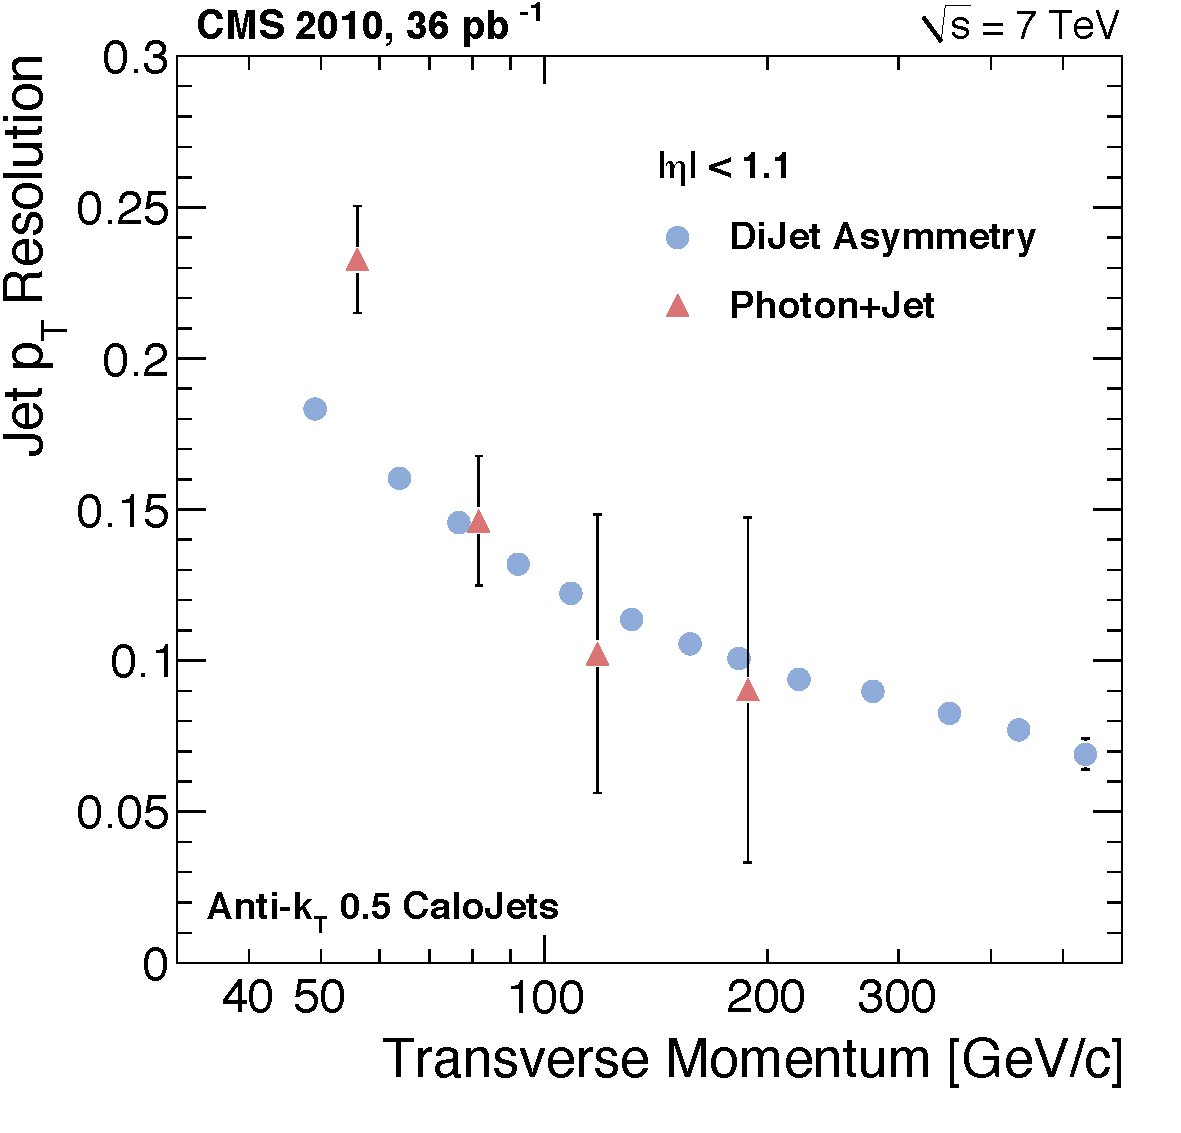
\includegraphics[width=0.45\textwidth]{Figures/JER/figs/res_photon/reso_dijet_gammajet_caloakt5}
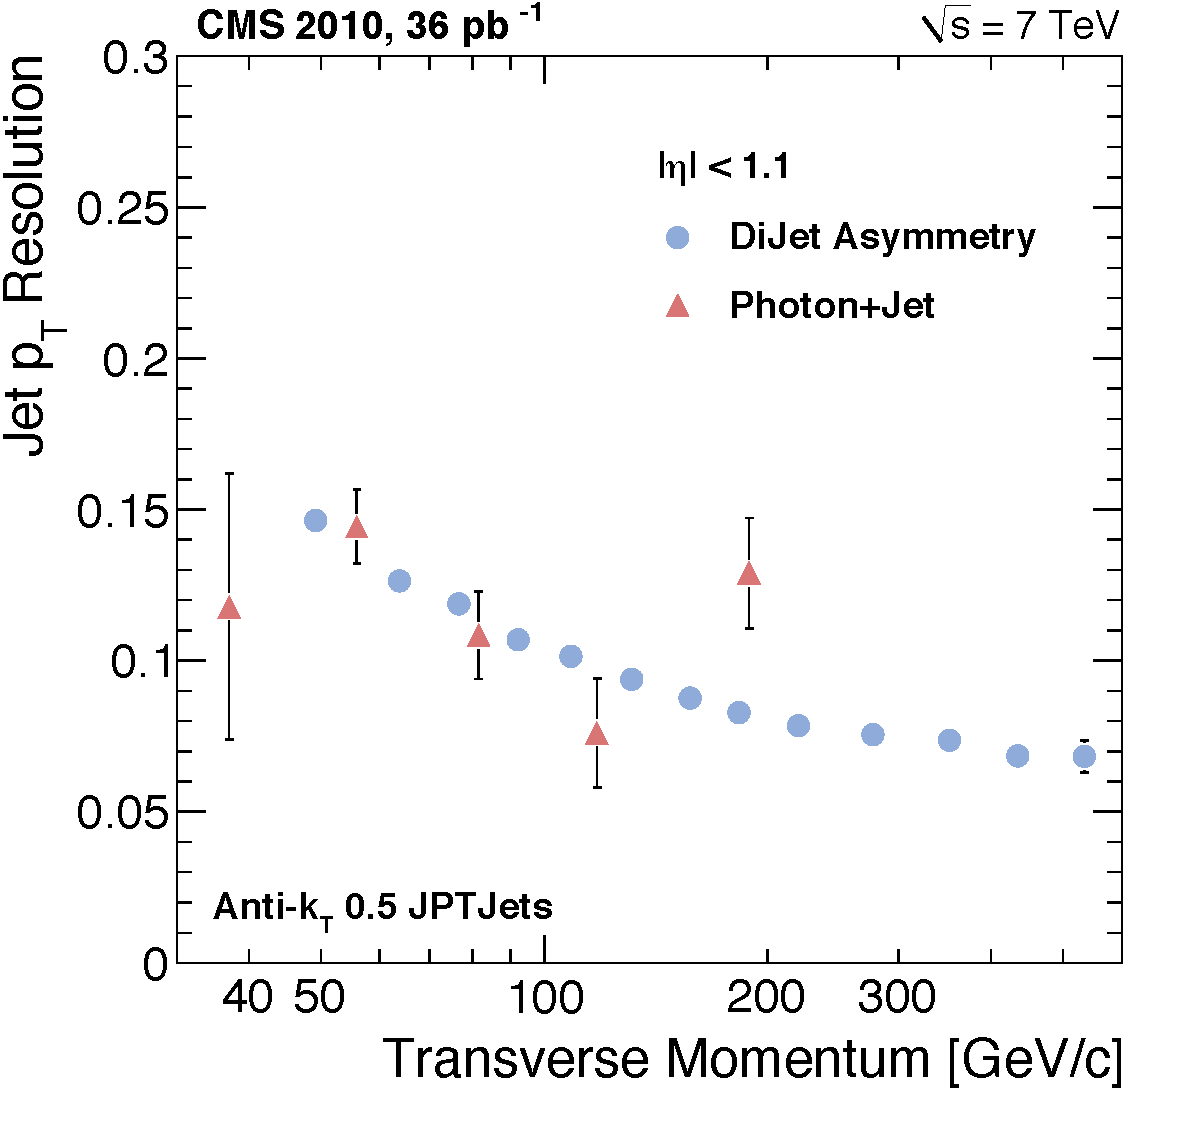
\includegraphics[width=0.45\textwidth]{Figures/JER/figs/res_photon/reso_dijet_gammajet_jptakt5}
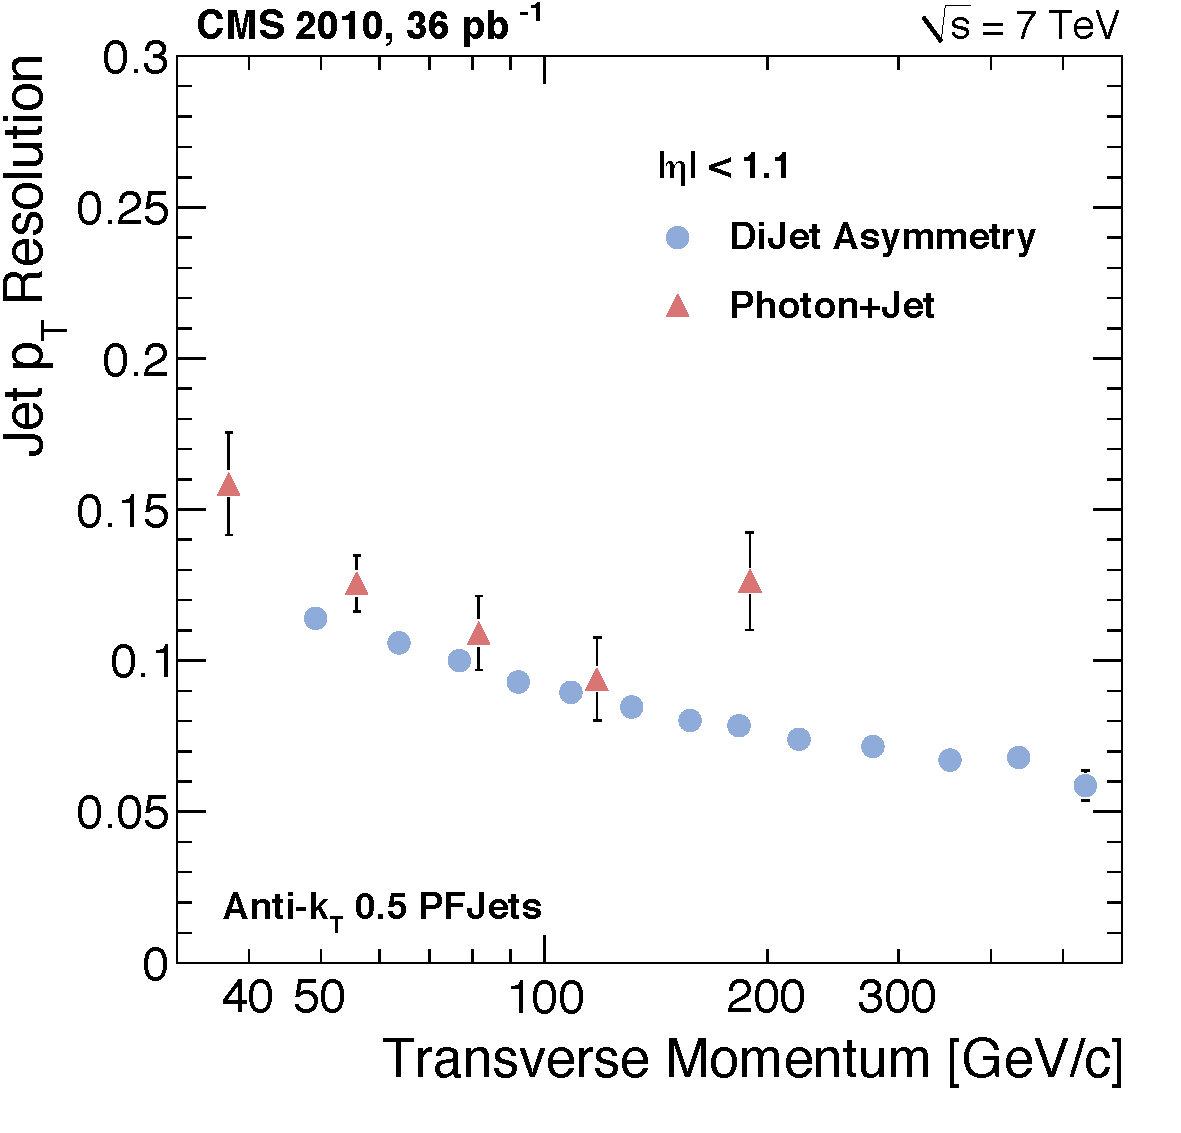
\includegraphics[width=0.45\textwidth]{Figures/JER/figs/res_photon/reso_dijet_gammajet_pfakt5}
\caption{Jet \pt resolutions from $\gamma+$jet (red triangular points) and dijet asymmetry (blue circular points) measurements, for CALO (top left), JPT (top right), and PF jets (bottom).}
\label{fig:gammajet_dijet}
\end{figure}

The complementary ``ratio'' method is based on taking the ratio of the data and MC intrinsic resolutions versus $\pt^{Jet2}/\pt^{\gamma}$ before the extrapolation. The intrinsic resolutions are first derived in data and MC, by subtracting in quadrature, from the total measured resolutions, the imbalance predicted in the simulation. The strength of the method is that the extrapolation fit is performed only once, and that the fitted observable, as estimator of the ratio of data and MC intrinsic resolutions, is expected to be a constant function of $\pt^{Jet2}/\pt^{\gamma}$. The intrinsic resolution derived in data is confirmed to be flat vs. $\pt^{Jet2}/\pt^{\gamma}$, as expected, providing a test of the procedure. Any deviation from a flat dependence would have indicated a limitation of the simulation to model the imbalance in the data. The results for the ratio are consistent with the constant $\pt^{Jet2}/\pt^{\gamma}$ behaviour and therefore a simple constant fit has been performed in bins of \pt and $\eta$. Systematic uncertainties due to variation of the extrapolation fit range and the uncertainty of jet energy corrections have been evaluated, adding up to $\pm (3-4)\%$ for the ratio. An additional uncertainty of $\pm (2-4)\%$ is assigned to the ratio, due to the assumption that the MC simulation correctly models the imbalance in data. This  uncertainty is evaluated by varying the relevant features at generator level, namely, the modeling of hadronization, treatment of multiple-parton final states and modeling of the $k_T$-kick. The direct and ratio methods are consistent with each other within uncertainties. The statistical errors on the results from the ratio method are smaller than 
from the direct method, because of the fact that in the ratio method the imbalance is fixed to the MC-based result, while in  the direct method the parameter $m$, describing the imbalance part of the resolution, is free in the fits to data and MC samples.

The results from the ratio method are compared in Fig.~\ref{fig:ResolutionRatioSum} (left) to the results from the dijet samples (using the unbinned likelihood fits), as a function of \pt, in the barrel region. Since the two samples have different jet flavour 
compositions, the generator-level MC resolutions from the corresponding MC samples  have been compared and verified that the difference is within $3\%$. The dependence of the data/MC ratio on the flavour difference is expected to be $\sim 1\%$ under a conservative assumption of $30\%$ uncertainty on the modeling of the flavour composition in the simulation.  This component is included in the comparison of the data/MC ratio between the dijet and $\gamma +$jet samples.

Therefore, the two results are compared directly, without applying additional jet composition corrections. Both sets of points are fully consistent and have been combined in fits, using a constant function of \pt for each $\eta$ range. The $\eta$ dependence of the measured intrinsic resolution ratios is also shown in Fig.~\ref{fig:ResolutionRatioSum} (right).

\begin{figure}[htbp]
\begin{center}
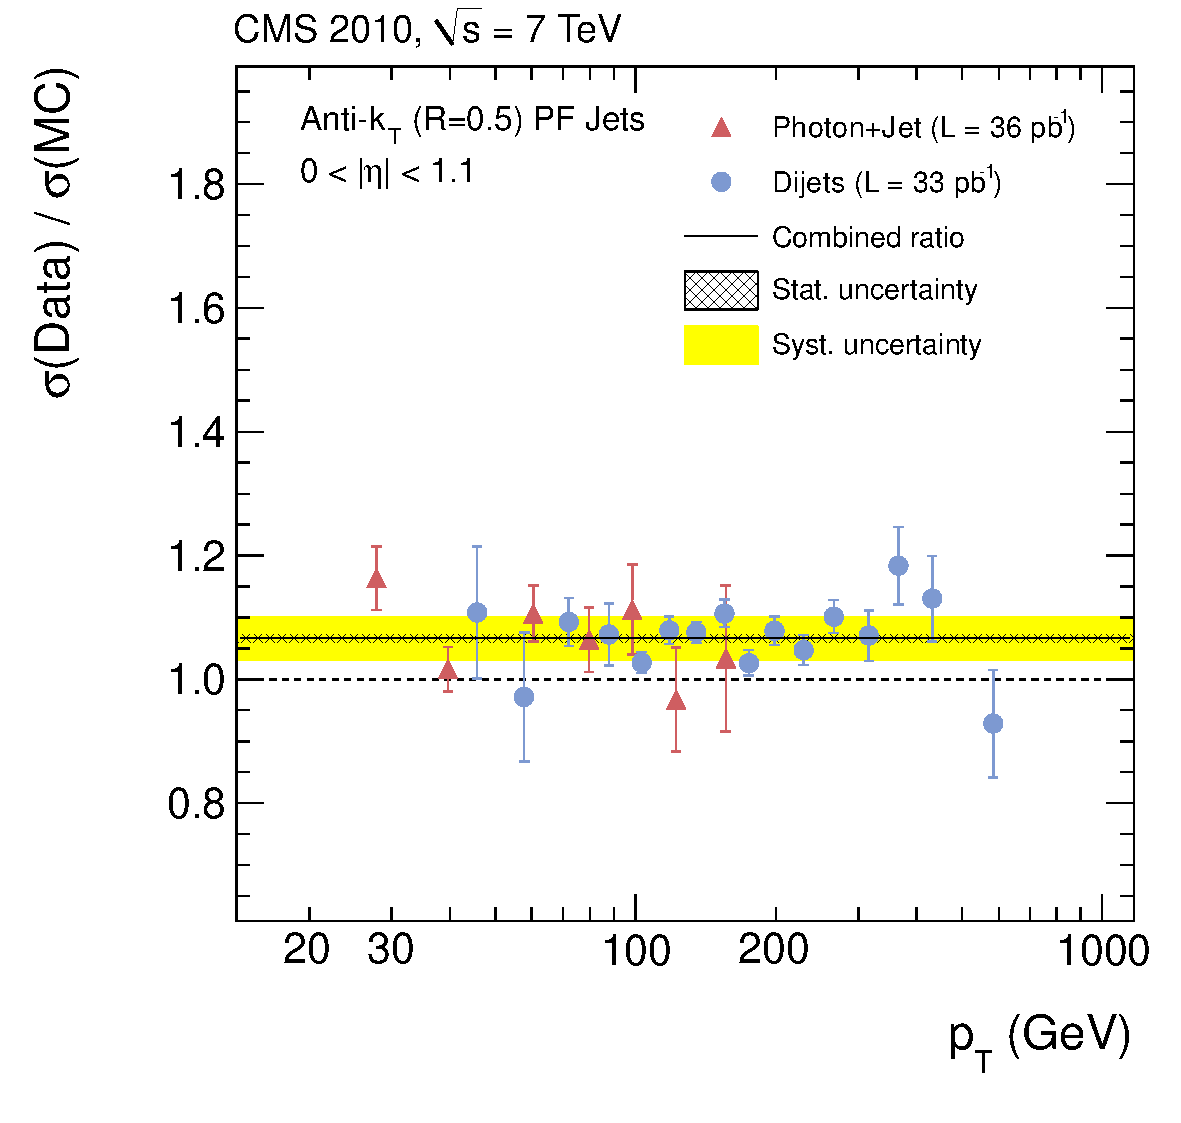
\includegraphics[width=0.49\textwidth]{Figures/JER/figs/res_photon/CombinedResolution_Eta0.pdf}
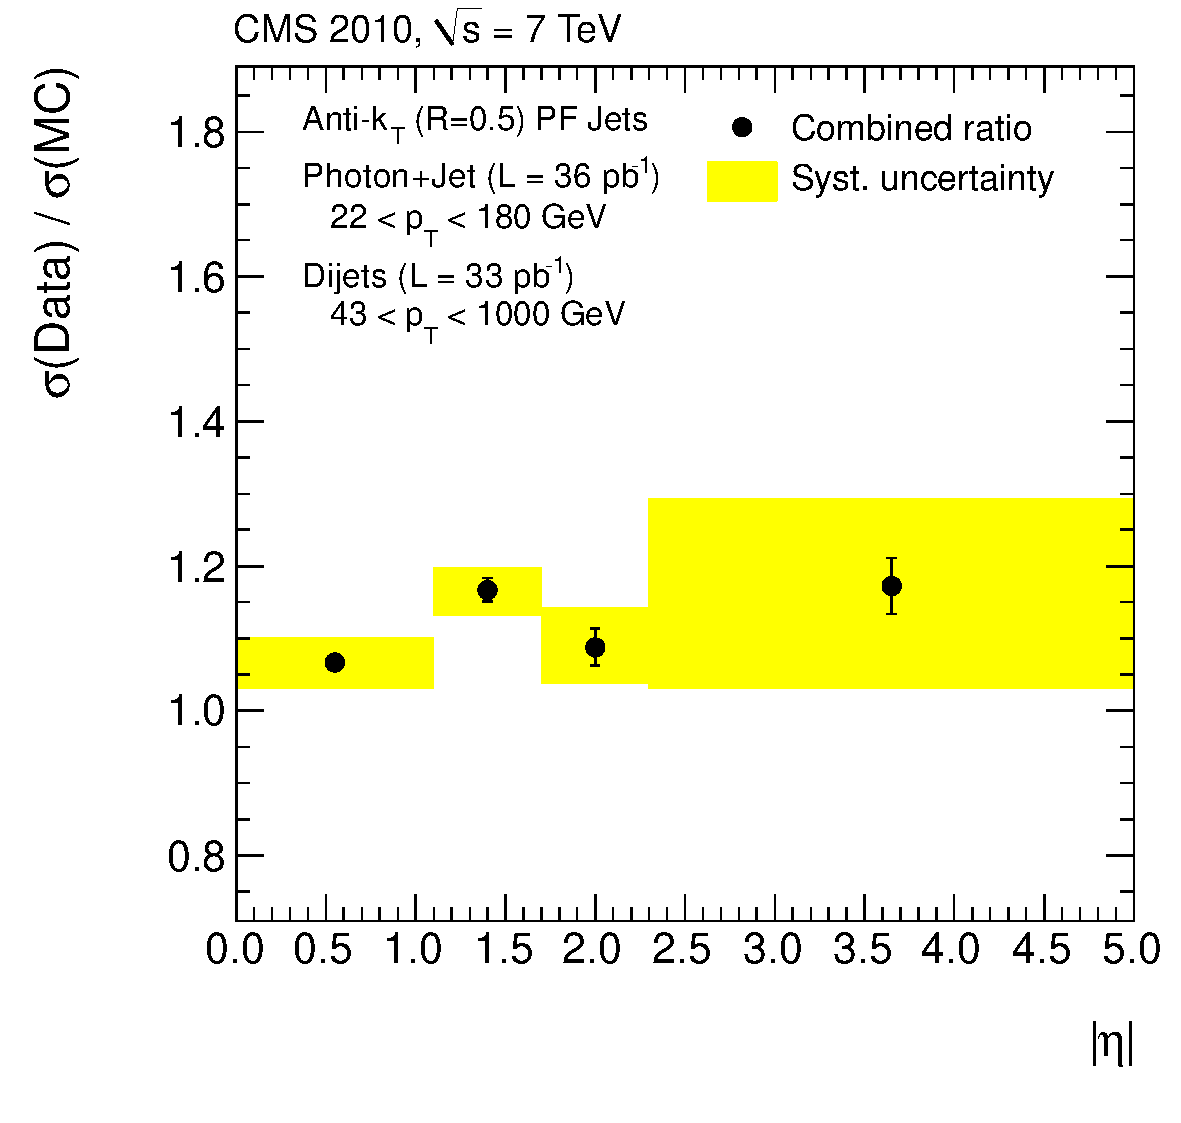
\includegraphics[width=0.49\textwidth]{Figures/JER/figs/res_photon/CombinedResolutionVsEta.pdf}
\end{center}
\caption[]{The ratio of jet \pt resolutions in data and MC samples vs. \pt, in $|\eta|<1.1$, from dijet and $\gamma+$jet samples; a combination fit to both  data sets is also shown (left). Results from the combination  fits vs. \pt in various $\eta$ ranges (right).}
\label{fig:ResolutionRatioSum}
\end{figure}

The results from the ratio method, as well as the results  from the dijet samples (using the unbinned likelihood fits), integrated over \pt and for all four different $|\eta|$ regions are illustrated in Table \ref{tab:ResFit:ScalingFactors}. As before, good agreement is observed between the two methods, within the statistical and systematic uncertainties. The quoted uncertainties for the dijet analysis combine the systematic uncertainties assigned to the extrapolation procedure,  the particle-level imbalance correction, the jet-energy-scale correction, and the particle-level dijet \pt spectrum. 

\begin{table}[ht]
  \caption{Ratios of the resolution measured in data and simulation for different jet $\eta$ ranges using the unbinned likelihood fits in dijet samples; the last column gives the ratio for PF jets from $\gamma$+jet samples for comparison. Stated are the statistical uncertainties from the fit and the upper and lower systematic uncertainties.}
  \begin{center}
\begin{tabular}[ht]{ccccc}
\hline
$|\eta|$ bin & Ratio CALO Jets & Ratio JPT Jets & Ratio PF Jets & Ratio PF Jets in $\gamma$+jet\\
\hline
\raisebox {0mm} [5mm] [3mm] {
0.0 -- 1.1} & $1.088 \pm 0.007 ^{+ 0.076}_{- 0.075}$ & $1.087 \pm 0.006^{+0.080}_{-0.078}$ &$1.066 \pm 0.007 ^{+
0.074}_{ - 0.072}$& $1.07\pm 0.020^{+0.024}_{- 0.033}$ \\
\raisebox {0mm} [3mm] [3mm] {
1.1 -- 1.7} & $1.139 \pm 0.019 ^{+ 0.084}_{ - 0.084}$ & $1.213 \pm 0.015^{+0.081}_{-0.080}$ &$1.191 \pm 0.019 ^{+
0.064}_{ - 0.062}$& $1.10 \pm 0.031^{+0.031}_{-0.039}$ \\
\raisebox {0mm} [3mm] [3mm] {
1.7 -- 2.3} & $1.082 \pm 0.030 ^{+ 0.140}_{ - 0.139}$ & $1.018 \pm 0.021^{+0.071}_{-0.071}$ &$1.096 \pm 0.030 ^{+
0.089}_{ - 0.085}$& $1.07 \pm 0.048^{+0.056}_{-0.047}$ \\
\raisebox {0mm} [3mm] [3mm] {
2.3 -- 5.0} & $1.065 \pm 0.042 ^{+ 0.237}_{ - 0.235}$ & $1.068 \pm 0.036^{+0.139}_{-0.139}$ &$1.166 \pm 0.050 ^{+
0.198}_{ - 0.199}$& $1.18 \pm 0.062^{+0.043}_{-0.072}$ \\
\hline
\end{tabular}
  \end{center}
  \label{tab:ResFit:ScalingFactors}
\end{table}

